% LaTeX source for ``Python for Informatics: Exploring Information''
% Copyright (c)  2010-  Charles R. Severance, All Rights Reserved

\chapter{Ficheros}

\index{fichero}
\index{archivo}
\index{tipo!file}


\section{Persistencia}

\index{persistencia}
\index{memoria!secundaria}

Hasta ahora, hemos aprendido cómo escribir programas y comunicar
nuestras intenciones a la {\bf Unidad Central de Procesamiento} usando ejecución
condicional, funciones e iteraciones. Hemos aprendido cómo
crear y usar estructuras de datos en la {\bf Memoria Principal}. La CPU
y la memoria son los lugares donde nuestro software trabaja y funciona. Ahí es
donde se desarrolla toda la ``inteligencia''.

Pero si te acuerdas de nuestra discusión sobre arquitectura del hardware,
una vez que la corriente se interrumpe, cualquier cosa almacenada tanto
en la CPU como en la memoria principal se borra. Así que hasta ahora, nuestros
programas ha sido sólo fugaces y divertidos ejercicios para aprender Python.

\beforefig
\centerline{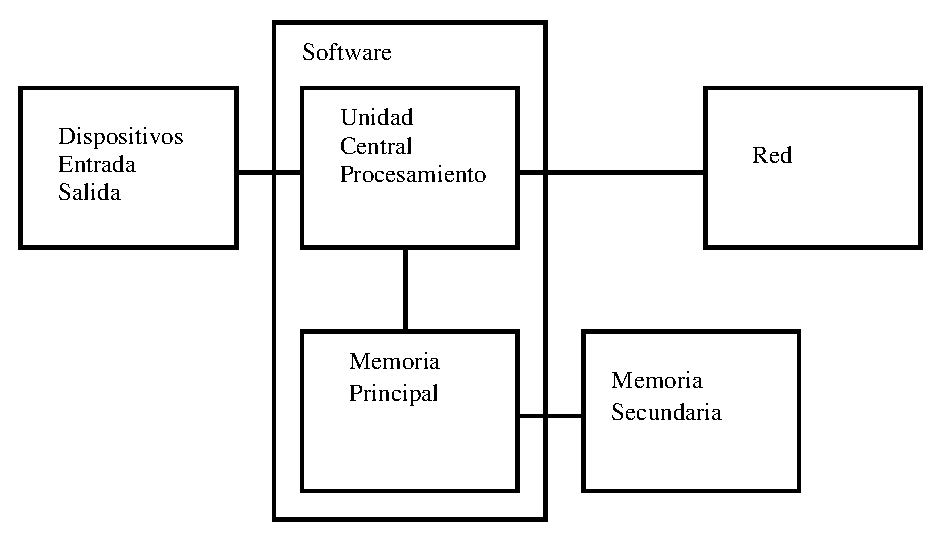
\includegraphics[height=2.50in]{figs2/arch3.eps}}
\afterfig

En este capítulo, comenzaremos a trabajar con la {\bf Memoria Secundaria}
(o ficheros, o archivos).
La memoria secundaria no se borra aunque se interrumpa la corriente.
Incluso, en el caso de una unidad flash USB, los
datos que escribamos desde nuestros programas pueden ser retirados
del sistema y transportados a otro equipo.

En primer lugar nos centraremos en leer y escribir ficheros de texto,
como los que se crean usando un editor de texto cualquiera. Más tarde veremos cómo
trabajar con archivos de bases de datos, que son ficheros binarios diseñados
específicamente para ser leídos y escritos mediante software de manejo de bases de datos.

\section{Apertura de ficheros}
\index{fichero!abrir}
\index{open, función}
\index{función!open}

Cuando se desea leer o escribir en un archivo (nos referimos en el disco duro), primero
debemos {\bf abrir} el fichero. Al abrir el fichero nos comunicamos con el sistema
operativo, que sabe dónde se encuentran almacenados los datos de cada archivo. Cuando se
abre un fichero, se está pidiendo al sistema operativo que lo busque por su nombre
y se asegure de que existe. En este ejemplo, abrimos el fichero
{\tt mbox.txt}, que debería estar guardado en la misma carpeta en la que te
encontrabas cuando iniciaste Python.
Puedes descargar el fichero desde
\url{www.py4inf.com/code/mbox.txt}

\beforeverb
\begin{verbatim}
>>> manf = open('mbox.txt')
>>> print manf
<open file 'mbox.txt', mode 'r' at 0x1005088b0>
\end{verbatim}
\afterverb
%
\index{manejador de fichero}
Si la {\tt apertura} tiene éxito, el sistema operativo nos devuelve un
{\bf manejador de fichero} ({\tt file handle}). El manejador de fichero no son los datos que
contiene en realidad el archivo, sino que se trata de un ``manejador'' ({\tt handle}) que se
puede utilizar para leer esos datos. Sólo obtendrás el manejador si el fichero especificado
existe y además dispones de los permisos apropiados para poder leerlo.

\beforefig
\centerline{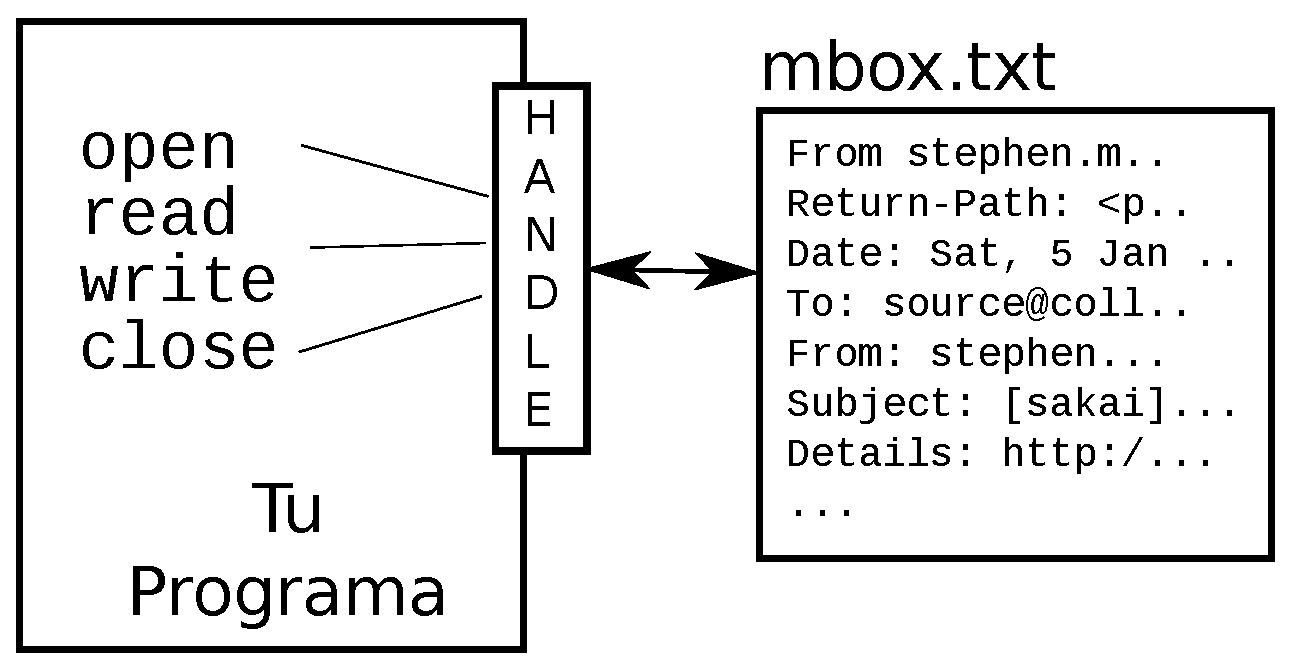
\includegraphics[height=1.75in]{figs2/handle.eps}}
\afterfig

Si el fichero no existe, {\tt open} fallará con un traceback, y no obtendrás
ningún manejador para poder acceder a su contenido:

\beforeverb
\begin{verbatim}
>>> manf = open('cosas.txt')
Traceback (most recent call last):
  File "<stdin>", line 1, in <module>
IOError: [Errno 2] No such file or directory: 'cosas.txt'
\end{verbatim}
\afterverb
%
Más adelante usaremos {\tt try} y {\tt except} para controlar con más
elegancia la situación cuando intentemos abrir un archivo
que no existe.

\section{Ficheros de texto y líneas}

Un fichero de texto puede ser considerado una secuencia de líneas, de igual
modo que una cadena en Python puede ser considerada una secuencia de caracteres.
Por ejemplo, ésta es una muestra de un fichero de texto que guarda la actividad de correos
de varias personas en el equipo de desarrollo de un proyecto de código abierto:

\beforeverb
\begin{alltt}
From stephen.marquard@uct.ac.za Sat Jan  5 09:14:16 2008
Return-Path: <postmaster@collab.sakaiproject.org>
Date: Sat, 5 Jan 2008 09:12:18 -0500
To: source@collab.sakaiproject.org
From: stephen.marquard@uct.ac.za
Subject: [sakai] svn commit: r39772 - content/branches/
Details: http://source.sakaiproject.org/viewsvn/?view=rev\&rev=39772
...
\end{alltt}
\afterverb

El fichero completo de interacciones de correo está disponible en
\url{www.py4inf.com/code/mbox.txt} 
y una versión más reducida se puede encontrar en
\url{www.py4inf.com/code/mbox-short.txt}.
Estos ficheros tienen un formato estándar, diseñado para archivos que contienen
múltiples mensajes de correo. Las líneas que comienzan con
``From '' separan los mensajes, y las líneas que comienzan con
``From:'' son parte de los mensajes.
Para tener más información sobre el formato mbox, consulta
\url{en.wikipedia.org/wiki/Mbox}. 

Para dividir el archivo en líneas, existe un carácter especial que
representa el ``final de línea'', llamado {\bf salto de línea} ({\tt newline}).

\index{salto de línea}
En Python, el carácter {\bf salto de línea} se representa por barra invertida-n en
las cadenas. A pesar de que parezcan dos caracteres, se
trata en realidad de uno sólo. Cuando revisamos la variable introduciendo
``cosa'' en el intérprete, nos mostrará el \verb"\n" en la cadena,
pero cuando usemos {\tt print} para mostrar la cadena, veremos cómo ésta
aparece dividida en dos líneas por el carácter de salto de línea.

\beforeverb
\begin{verbatim}
>>> cosa = '¡Hola\nMundo!'
>>> cosa
'¡Hola\nMundo!'
>>> print cosa
¡Hola
Mundo!
>>> cosa = 'X\nY'
>>> print cosa
X
Y
>>> len(cosa)
3
\end{verbatim}
\afterverb
%

También puedes observar que la longitud de la cadena \verb"'X\nY'" es de \emph{tres}
caracteres, porque el carácter de salto de línea se cuenta como uno sólo.

Por tanto, cuando miremos a las líneas de un fichero, tendremos que \emph{imaginarnos}
que existe un carácter especial invisible llamado salto de línea al
final de cada línea, que marca donde termina la misma y comienza la siguiente.

% \beforeverb
% \begin{alltt}
% From stephen.marquard@uct.ac.za Sat Jan  5 09:14:16 2008\verb"\n"\\
% Return-Path: <postmaster@collab.sakaiproject.org>\verb"\n"\\
% Date: Sat, 5 Jan 2008 09:12:18 -0500\verb"\n"\\
% To: source@collab.sakaiproject.org\verb"\n"\\
% From: stephen.marquard@uct.ac.za\verb"\n"\\
% Subject: [sakai] svn commit: r39772 - content/branches/\verb"\n"\\
% Details: http://source.sakaiproject.org/viewsvn/?view=rev\&rev=39772\verb"\n"\\
% ...
% \end{alltt}
% \afterverb

De modo que el carácter de salto de línea separa los caracteres
del fichero en líneas.

\section{Lectura de ficheros}

\index{fichero!lectura}
\index{contador}
A pesar de que el {\bf manejador de fichero} no contiene los datos del archivo,
es bastante fácil construir un bucle {\tt for} para ir leyendo
y contabilizando cada una de las líneas de un fichero:

\beforeverb
\begin{verbatim}
manf = open('mbox.txt')
contador = 0
for linea in manf:
    contador = contador + 1
print 'Líneas contabilizadas:', contador

python open.py 
Line Count: 132045
\end{verbatim}
\afterverb
%
Podemos usar el manejador del fichero como una secuencia en nuestro bucle {\tt for}.
El bucle {\tt for} simplemente cuenta el número de líneas del
fichero y lo muestra en pantalla. La traducción aproximada de ese bucle
al español es: ``para cada línea del fichero representado por el
manejador, añade una unidad a la variable {\tt contador}''.

La razón de que la función {\tt open} no lea el archivo completo
es que el fichero puede ser bastante extenso, con muchos gigabytes de datos.
La sentencia {\tt open} emplea la misma cantidad de tiempo independientemente del
tamaño del archivo. En realidad es el bucle {\tt for} el que hace que
los datos sean leídos desde el fichero.

Cuando el archivo se lee de este modo, usando un bucle {\tt for}, Python
se encarga de dividir los datos del fichero en líneas independientes, usando
el carácter de salto de línea. Python lee cada línea hasta el
salto de línea e incluye
el propio salto de línea como último carácter en la variable {\tt linea} para
cada iteración del bucle {\tt for}.

Como el bucle {\tt for} lee los datos línea a línea, puede
leer y contar las líneas de forma eficiente en ficheros muy extensos sin
agotar la memoria de almacenamiento de datos. El programa anterior puede
contar las líneas de ficheros de cualquier tamaño usando muy poca memoria,
ya que cada línea es leída, contabilizada y luego descartada.

Si sabes que el fichero es relativamente pequeño comparado con el tamaño de
tu memoria principal, puedes leer el fichero completo en una cadena
usando el método {\tt read} sobre el manejador del fichero.

\beforeverb
\begin{verbatim}
>>> manf = open('mbox-short.txt')
>>> ent = manf.read()
>>> print len(ent)
94626
>>> print ent[:20]
From stephen.marquar
\end{verbatim}
\afterverb
%
En este ejemplo, el contenido completo (los 94.626 caracteres)
del fichero {\tt mbox-short.txt} se leen directamente dentro de la variable
{\tt ent}. Usamos luego rebanado de cadenas para imprimir en pantalla
los primeros 20 caracteres de la cadena de datos almacenada en {\tt ent}.

Cuando el archivo se lee de esta manera, todos los caracteres incluyendo
las líneas completas y los saltos de línea forman parte de una gran cadena
que se guarda en la variable {\bf ent}.
Recuerda que esta forma de uso de la función {\tt open} sólo debe utilizarse
si el fichero de datos cabe holgadamente en la memoria principal
de tu equipo.

Si el fichero es demasiado grande para caber en la memoria principal, deberías
hacer que tu programa leyera el archivo en bloques, usando un bucle
{\tt for} o {\tt while}.

\section{Búsqueda dentro de un fichero}

Cuando se buscan datos dentro de un fichero, un
diseño muy común consiste en ir leyendo el archivo completo, ignorando
la mayoría de las líneas y procesando únicamente aquellas que cumplen alguna condición
particular. Es posible combinar ese diseño de lectura de ficheros con los métodos de cadena
para construir un mecanismo simple de búsqueda.

\index{filtrado, patrón}
\index{patrón!de filtrado}
Por ejemplo, si queremos leer un fichero y mostrar unicamente las líneas
que comienzan con el prefijo ``From:'', podemos usar el
método de cadena {\bf startwith} para seleccionar solamente aquellas líneas con
el prefijo deseado:

\beforeverb
\begin{verbatim}
manf = open('mbox-short.txt')
for linea in manf:
    if linea.startswith('From:') :
        print linea
\end{verbatim}
\afterverb
%
Cuando se hace funcionar el programa, obtenemos la siguiente salida:

\beforeverb
\begin{verbatim}
From: stephen.marquard@uct.ac.za

From: louis@media.berkeley.edu

From: zqian@umich.edu

From: rjlowe@iupui.edu
...
\end{verbatim}
\afterverb
%
La salida parece ser correcta, ya que las únicas líneas que vemos son aquellas
que comienzan por ``From:''. Pero, ¿por qué estamos viendo líneas extra
vacías? Esto se debe al carácter invisible de {\bf salto de línea}.
Cada una de las líneas termina con un salto de línea, de modo que la sentencia
{\tt print} imprime la cadena que está en la variable {\bf linea} y que
incluye un salto de línea, y a continuación {\tt print} añade \emph{otro} salto de línea,
cuyo resultado es el efecto de doble espaciado que podemos ver.

Podríamos usar rebanado de líneas para imprimir todo menos el último carácter, pero
un enfoque más sencillo consiste en usar el método {\bf rstrip}, que retira
los espacios en blanco de la parte derecha de una cadena, como se muestra a continuación:

\beforeverb
\begin{verbatim}
manf = open('mbox-short.txt')
for linea in manf:
    linea = linea.rstrip()
    if linea.startswith('From:') :
        print linea
\end{verbatim}
\afterverb
%
Cuando hacemos funcionar el programa, obtenemos la siguiente salida:

\beforeverb
\begin{verbatim}
From: stephen.marquard@uct.ac.za
From: louis@media.berkeley.edu
From: zqian@umich.edu
From: rjlowe@iupui.edu
From: zqian@umich.edu
From: rjlowe@iupui.edu
From: cwen@iupui.edu
...
\end{verbatim}
\afterverb
%
A medida que los programas de procesado de archivos se van volviendo más complejos, tal vez
prefieras estructurar los bucles de búsqueda usando {\tt continue}. La idea básica
del bucle de búsqueda es que estamos localizando líneas ``interesantes'',
en realidad saltándonos aquellas que ``no nos interesan''. Y a continuación, cuando
encontramos una línea interesante, hacemos algo con ella.

Podemos estructurar el bucle para usar ese
diseño y saltar las líneas que no nos interesan, de este modo:

\beforeverb
\begin{verbatim}
manf = open('mbox-short.txt')
for linea in manf:
    linea = linea.rstrip()
    # Saltar 'líneas que no nos interesan'
    if not linea.startswith('From:') :
        continue
    # Procesar nuestra línea 'interesante'
    print linea
\end{verbatim}
\afterverb
%
La salida del programa es la misma. Traduciendo, las
líneas que no nos interesan son aquellas que no comienzan
por ``From:'', de modo que las saltamos usando {\tt continue}.
En cambio las líneas ``interesantes'' (es decir, aquellas que comienzan por ``From:''),
procedemos a procesarlas.

Podemos usar el método {\tt find} para simular una búsqueda como la de
un editor que texto, que localice aquellas líneas que contengan la cadena buscada
en cualquier punto de las mismas.
Dado que {\tt find} comprueba la aparición de una cadena dentro de otra
y devuelve la posición de la cadena o -1 si no la ha encontrado,
podemos escribir el bucle siguiente para mostrar aquellas líneas
que contienen la cadena ``@uct.ac.za'' (es decir, las que proceden de la Universidad
de Cape Town en Sudáfrica):

\beforeverb
\begin{verbatim}
manf = open('mbox-short.txt')
for linea in manf:
    linea = linea.rstrip()
    if linea.find('@uct.ac.za') == -1 : 
        continue
    print linea
\end{verbatim}
\afterverb
%
Que produce la salida siguiente:

\beforeverb
\begin{verbatim}
From stephen.marquard@uct.ac.za Sat Jan  5 09:14:16 2008
X-Authentication-Warning: set sender to stephen.marquard@uct.ac.za using -f
From: stephen.marquard@uct.ac.za
Author: stephen.marquard@uct.ac.za
From david.horwitz@uct.ac.za Fri Jan  4 07:02:32 2008
X-Authentication-Warning: set sender to david.horwitz@uct.ac.za using -f
From: david.horwitz@uct.ac.za
Author: david.horwitz@uct.ac.za
...
\end{verbatim}
\afterverb
%

\section{Permitiendo al usuario elegir el nombre del fichero}

Lo más probable es que no nos apetezca editar nuestro código Python
cada vez que queramos procesar un archivo diferente. Sería
más útil pedir al usuario que introdujera una cadena con el nombre del fichero
cada vez que el programa funcione, de modo que se pueda usar nuestro
programa sobre ficheros diferentes sin tener que cambiar el código Python.

Esto es bastante sencillo de hacer, pidiendo el nombre del fichero al
usuario mediante el uso de \verb"raw_input", como se muestra a continuación:

\beforeverb
\begin{verbatim}
nombref = raw_input('Introduzca el nombre del fichero: ')
manf = open(nombref)
contador = 0
for linea in manf:
    if linea.startswith('Subject:') :
        contador = contador + 1
print 'Hay', contador, 'líneas subject en', nombref
\end{verbatim}
\afterverb
%
Pedimos el nombre del fichero al usuario, lo guardamos en una variable
llamada {\tt nombref} y abrimos ese fichero. Ahora ya podemos hacer funcionar
el programa repetidamente con distintos ficheros.

\beforeverb
\begin{verbatim}
python search6.py 
Introduzca el nombre del fichero: mbox.txt
Hay 1797 líneas subject en mbox.txt

python search6.py 
Introduzca el nombre del fichero: mbox-short.txt
Hay 27 líneas subject en mbox-short.txt
\end{verbatim}
\afterverb
%
Antes de asomarte a la siguiente sección, échale un vistazo al programa anterior
y pregúntate a ti mismo: ``¿Qué podría salir mal aquí?'', o ``¿Qué podría hacer
nuestro simpático usuario que provoque que nuestro bonito programita
termine sin gracia, con un tracebak, haciéndonos parecer menos geniales
ante los usuarios?

\section{Uso de {\tt try, except,} y {\tt open}}

Te avisé que no te asomases. Esta es tu última oportunidad.

¿Qué ocurre si nuestro usuario escribe algo que no es un nombre de fichero?

\beforeverb
\begin{verbatim}
python search6.py 
Introduzca el nombre del fichero: perdido.txt
Traceback (most recent call last):
  File "search6.py", line 2, in <module>
    manf = open(nombref)
IOError: [Errno 2] No such file or directory: 'perdido.txt'

python search6.py 
Introduzca el nombre del fichero: na na boo boo
Traceback (most recent call last):
  File "search6.py", line 2, in <module>
    manf = open(nombref)
IOError: [Errno 2] No such file or directory: 'na na boo boo'
\end{verbatim}
\afterverb
%
No te rías, los usuarios harán de vez en cuando todo lo que puedan por estropear
tus programas---ya sea a propósito o con malas intenciones.
De hecho, una parte importante de cualquier equipo de desarrollo de software
es una persona o grupo llamado {\bf Controlador de Calidad}
(o QA por sus siglas en inglés), cuyo trabajo principal es hacer las cosas más disparatadas
posibles para intentar hacer fallar el software que el programador ha creado.

\index{Controlador de Calidad}
\index{QA}
El equipo de QA es el responsable de encontrar los defectos en los programas antes
de que éstos se entreguen a los usuarios finales, que pueden estar comprando el
software o pagando su salario a los que escriben el software. De modo que el equipo QA
es el mejor amigo del programador.

\index{try, sentencia}
\index{sentencia!try}
\index{open, función}
\index{función!open}
\index{exception!IOError}
\index{IOError}
Así que ahora que hemos visto el defecto en el programa, podemos solucionarlo
de forma elegante usando la estructura {\tt try}/{\tt except}. Debemos asumir que la llamada
a {\tt open} puede fallar y añadir código de recuperación para ese fallo,
como se muestra a continuación:

\beforeverb
\begin{verbatim}
nombref = raw_input('Introduzca el nombre del fichero: ')
try:
    manf = open(nombref)
except:
    print 'No se pudo abrir el fichero:', nombref
    exit()

contador = 0
for linea in manf:
    if linea.startswith('Subject:') : 
        contador = contador + 1
print 'Hay', contador, 'líneas subject en', nombref
\end{verbatim}
\afterverb
%
La función {\tt exit} hace finalizar el programa. Se trata de una función
que llamamos sin retorno. Ahora cuando el usuario (o
el equipo de QA) escriba tonterías o nombres de archivo incorrectos,
los ``capturaremos'' y recuperaremos el control del programa con elegancia:

\beforeverb
\begin{verbatim}
python search7.py
Introduzca el nombre del fichero: mbox.txt
Hay 1797 líneas subject en mbox.txt

python search7.py
Introduzca el nombre del fichero: na na boo boo
No se pudo abrir el fichero: na na boo boo
\end{verbatim}
\afterverb
%
\index{Pythónico}
La protección de la llamada a {\tt open} es un buen ejemplo
del uso correcto de {\tt try}
y {\tt except} en un programa Python. Se utiliza el término
``Pythónico'' cuando estamos haciendo algo al ``modo
Python''. Podríamos decir que el ejemplo de arriba es
el modo Pythónico de abrir un archivo.

Una vez que adquieras más soltura en Python, puedes intercambiar
opiniones con otros programadores de Python para decidir
cual de dos soluciones equivalentes para un problema resulta
``más Pythónica''. La ambición de ser ``más Pythónico''
capta la idea de que programar es en parte ingeniería
y en parte arte. No siempre estamos interesados únicamente
en hacer que algo funcione sin más, también queremos que nuestra solución
sea elegante y que sea apreciada por su elegancia
por nuestros colegas.


\section{Escritura en ficheros}

\index{fichero!escritura}

Para escribir en un fichero, debes abrirlo usando el modo
\verb"'w'" (de {\tt write}) como segundo parámetro:

\beforeverb
\begin{verbatim}
>>> fsal = open('salida.txt', 'w')
>>> print fsal
<open file 'salida.txt', mode 'w' at 0xb7eb2410>
\end{verbatim}
\afterverb
%
Si el fichero ya existe, abrirlo en modo escritura eliminará
los datos antiguos y lo dejará completamente vacío, ¡así que ten cuidado!
Si el fichero no existe, se creará nuevo.

El método {\tt write} del objeto manejador del fichero
pone datos dentro del archivo.

\beforeverb
\begin{verbatim}
>>> linea1 = "Aquí está el zarzo,\n"
>>> fsal.write(linea1)
\end{verbatim}
\afterverb
%
\index{salto de línea}
El objeto fichero también realiza el seguimiento de la posición dentro del fichero, de modo
que si se llama a {\tt write} otra vez, añadirá los datos nuevos al final del archivo.

Deberemos asegurarnos de gestionar los finales de las líneas mientras
escribimos en el fichero, insertando explícitamente el carácter de salto
cuando queramos terminar una línea. La sentencia {\tt print}
añade un salto de línea automáticamente, pero el método
{\tt write} no lo hace a menos que se lo especifiquemos.

\beforeverb
\begin{verbatim}
>>> linea2 = 'el símbolo de nuestra tierra.\n'
>>> fsal.write(linea2)
\end{verbatim}
\afterverb
%
Cuando hayas terminado de escribir, debes cerrar el fichero
para asegurarte de que hasta el último bit de datos se escriba
físicamente en el disco, de modo que no se pierda si la corriente se interrumpe.

\beforeverb
\begin{verbatim}
>>> fsal.close()
\end{verbatim}
\afterverb
%
También se pueden cerrar los ficheros que se han abierto en modo lectura,
pero no es necesario que seamos muy estrictos con ello si solamente
estamos abriendo unos pocos archivos, ya que Python se asegura de que
todos los ficheros queden cerrados cuando el programa termina. En cambio, en el caso
de que estemos escribiendo ficheros, deberemos cerrarlos explícitamente
para no dejar nada al azar.

\index{close, método}
\index{método!close}


\section{Depuración}

\index{depuración}
\index{espacio en blanco}

Cuando estés leyendo y escribiendo archivos, puedes tener problemas
con los espacios en blanco. Estos errores pueden ser difíciles de depurar porque los espacios,
tabulaciones y saltos de línea normalmente son invisibles:

\beforeverb
\begin{verbatim}
>>> s = '1 2\t 3\n 4'
>>> print s
1 2	 3
 4
\end{verbatim}
\afterverb

\index{repr, función}
\index{función!repr}
\index{cadena!representación de}

La función interna {\tt repr} puede ayudarnos. Toma cualquier objeto como
argumento y devuelve una representación de cadena del objeto. En el caso
de las cadenas, representa los caracteres en blanco
con secuencias de barras invertidas:

\beforeverb
\begin{verbatim}
>>> print repr(s)
'1 2\t 3\n 4'
\end{verbatim}
\afterverb

Esto puede resultarnos útil a la hora de depurar.

Otro problema que puedes tener se debe a que los distintos sistemas
utilizan caracteres diferentes para indicar el final de una línea. Algunos
sistemas usan un salto de línea, representado por \verb"\n". Otros
usan un carácter de retorno, representado por \verb"\r". Otros usan ambos.
Si trasladas ficheros entre sistemas diferentes, esas inconsistencias
pueden causar problemas.

\index{final de línea, carácter de}

En la mayoría de los sistemas, existen aplicaciones para convertir de un
formato a otro. Puedes encontrarlos (y leer más acerca de este
problema) en \url{wikipedia.org/wiki/Newline}.  O, por supuesto, puedes
escribir tu propio programa.

% TBD - ¿¿¿No se ocupa Python de esto por nosotros????

\section{Glosario}

\begin{description}

\item[capturar (catch):] Evitar que una excepción haga terminar
un programa, usando las sentencias {\tt try} y {\tt except}.
\index{catch}
\index{capturar}

\item[Controlador de Calidad:] Una persona o equipo centrada en asegurar
la calidad del conjunto en un producto software.
Sus siglas en inglés son QA (Quality Assurance). El QA se encarga normalmente
de probar un producto e identificar sus problemas antes de que éste
sea lanzado.
\index{Controlador de Calidad}
\index{QA}

\item[fichero de texto:] Una secuencia de caracteres almacenados en un
medio de almacenamiento permanente, como un disco duro.
\index{fichero!de texto}

\item[Pythónico:] Una técnica que funciona de forma elegante en Python.
``Usar try y except y es la forma \emph{Pythónica} de restablecer un programa en
caso de intentar abrir archivos que no existen''.
\index{Pythónico}

\item[salto de línea:] Un carácter especial que se utiliza en los archivos y cadenas
para indicar el final de una línea.
\index{salto de línea}

\end{description}


\section{Ejercicios}

\begin{ex}
Escribe un programa que lea un fichero e imprima en pantalla su contenido
(línea a línea), todo en mayúsculas. La ejecución del programa debería
ser algo similar a esto:

\beforeverb
\begin{verbatim}
python shout.py
Introduzca el nombre del fichero: mbox-short.txt
FROM STEPHEN.MARQUARD@UCT.AC.ZA SAT JAN  5 09:14:16 2008
RETURN-PATH: <POSTMASTER@COLLAB.SAKAIPROJECT.ORG>
RECEIVED: FROM MURDER (MAIL.UMICH.EDU [141.211.14.90])
	 BY FRANKENSTEIN.MAIL.UMICH.EDU (CYRUS V2.3.8) WITH LMTPA;
	 SAT, 05 JAN 2008 09:14:16 -0500
\end{verbatim}
\afterverb
%
Puedes descargar el fichero desde
\url{www.py4inf.com/code/mbox-short.txt}
\end{ex}

\begin{ex}
Escribe un programa
que pida el nombre de un fichero y después lea ese fichero,
buscando líneas que tengan la forma:

\beforeverb
\begin{alltt}
X-DSPAM-Confidence: {\bf 0.8475}
\end{alltt}
\afterverb

Cuando encuentres una línea que comience por
``X-DSPAM-Confidence:'', separa esa línea para extraer
el número en punto flotante que figure en ella. Cuenta esas línea y
calcula también el total de los valores de probabilidad de spam (spam confidence)
de estas líneas. Cuando alcances el final del archivo, muestra en pantalla
el valor medio de probabilidad de spam.

\beforeverb
\begin{verbatim}
Introduzca el nombre del fichero: mbox.txt
Valor medio de probabilidad de spam: 0.894128046745

Introduzca el nombre del fichero: mbox-short.txt
Valor medio de probabilidad de spam: 0.750718518519
\end{verbatim}
\afterverb
%
Prueba tu programa con los archivos {\tt mbox.txt} y {\tt mbox-short.txt}.
\end{ex}


\begin{ex}
Algunas veces, cuando los programadores se aburren o quieren divertirse un poco,
añaden un inofensivo {\bf Huevo de Pascua} ({\tt Easter Egg}) en sus programas
(\url{es.wikipedia.org/wiki/Huevo_de_pascua_(virtual)}). Modifica el programa
que pide al usuario el nombre del fichero para que imprima un mensaje
divertido cuando el usuario escriba el nombre exacto ``na na boo boo''.
El programa debe comportarse normalmente con todos los demás ficheros,
tanto los que existan como los que no. A continuación, una muestra de la ejecución
del programa:

\beforeverb
\begin{verbatim}
python egg.py 
Introduzca el nombre del fichero:  mbox.txt
Hay 1797 líneas subject en mbox.txt

python egg.py 
Introduzca el nombre del fichero:  missing.tyxt
No se pudo abrir el fichero: missing.tyxt

python egg.py 
Introduzca el nombre del fichero: na na boo boo
NA NA BOO BOO PARA TI - ¡Te he pillado!
\end{verbatim}
\afterverb
%
No te estamos animando a poner Huevos de Pascua en tus
programa---se trata sólo de un ejercicio.

\end{ex}